\NewJ{Our goal is to enable the secure aggregation and elaboration of original, unaltered event logs from decentralized sources in dedicated environments that potentially lie beyond the individual organizations' information perimeter.
With this objective in mind, we devise the \Compo{Secure Miner} component, which is capable of securing data merge and processing by running certified code in an isolated execution vault. Thus, we decouple provisioning from treatment, and the two tasks can be carried out by distinct computing nodes.
Here, we introduce CONFINE's key components, with a special focus on the \Compo{Secure Miner}.}
\begin{figure}[t]
	\centering
	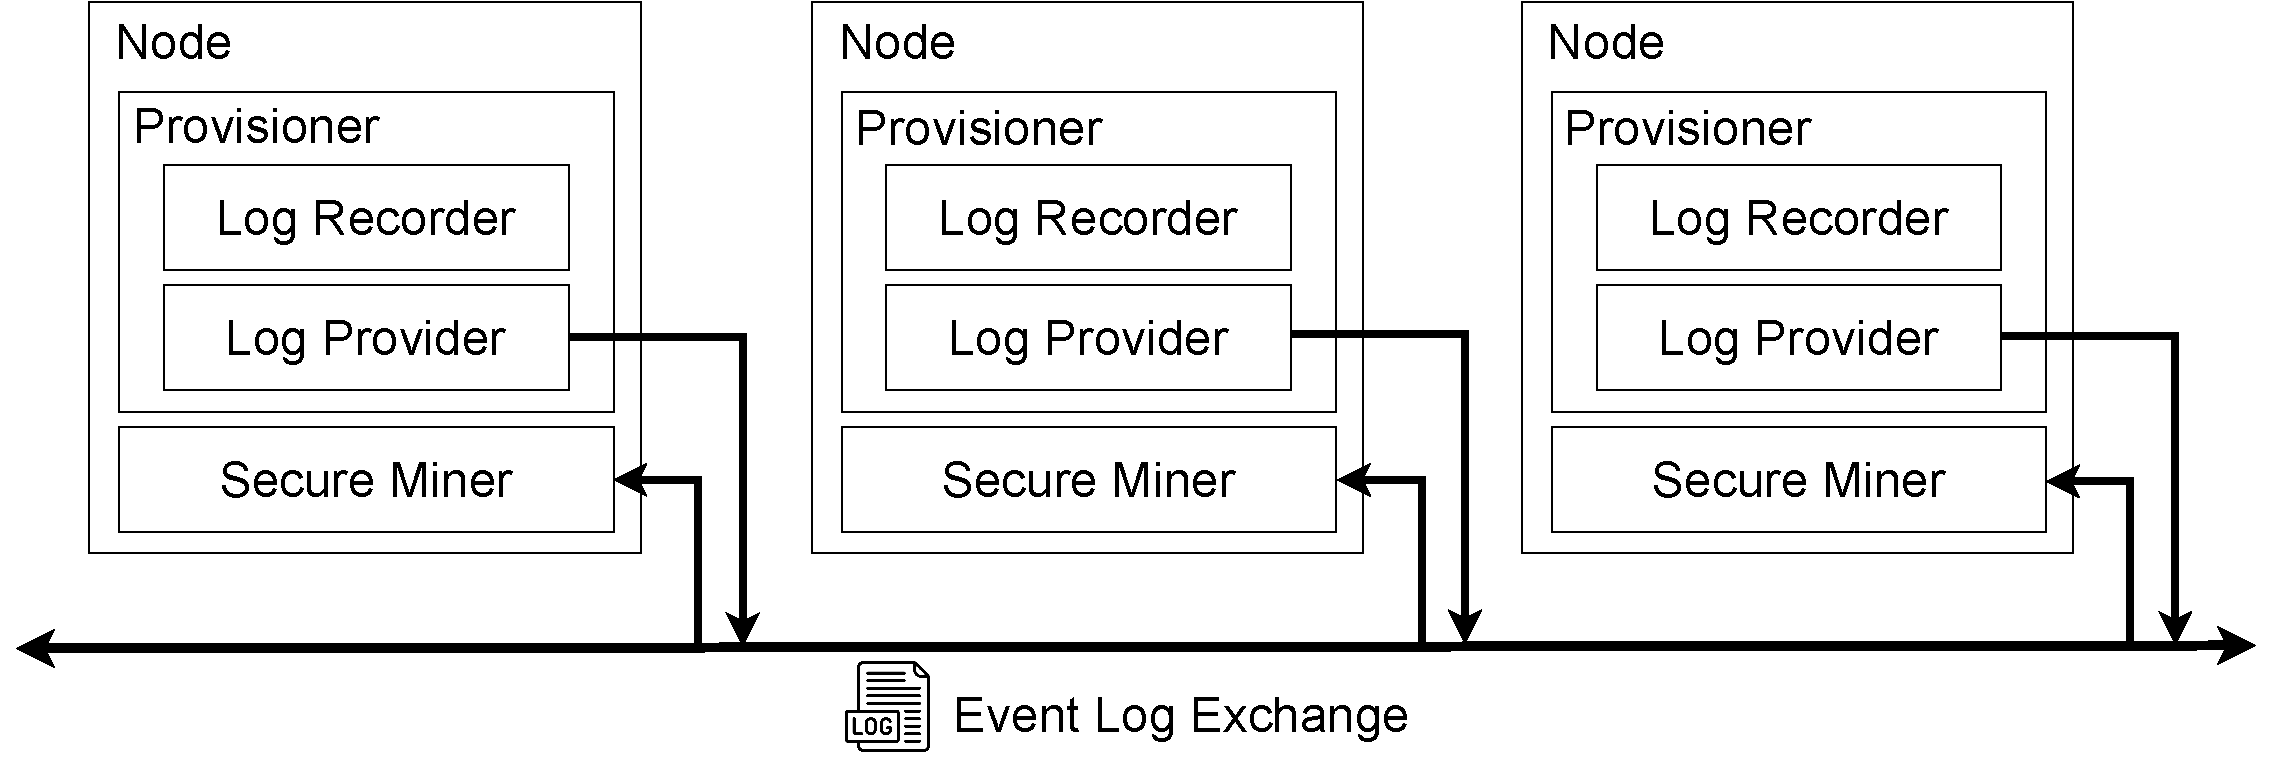
\includegraphics[width=1\linewidth]{content/figures/architecturediagram.pdf}
	\caption{The CONFINE high-level architecture}
	\label{fig:architecture_diagram}
\end{figure}


\noindent\textbf{The CONFINE architecture at large.} Our architecture involves different information systems running on multiple machines. An organization can take at least one of the following roles: 
\begin{inparadesc}
%\item[provisioning] if it delivers local event logs to be collaboratively mined;
%\item[mining] if it applies process mining algorithms using event logs retrieved from provisioners.
\item[provisioning] \NewJ{if it delivers local event logs to be collaboratively mined} (as per \cref{def:provisioner});
\item[miner] if it applies process mining algorithms using event logs retrieved from provisioners.
\end{inparadesc}
In \cref{fig:architecture_diagram}, we propose the high-level schematization of the CONFINE framework.
In our solution, every organization hosts one or more nodes hosting components (the names of which will henceforth be formatted with a \Compo{teletype} font). Depending on the played role, nodes come endowed with a \Compo{Provisioner} or a \Compo{Secure Miner} component, or both. The \Compo{Provisioner} component consists of the following two main sub-components. The \begin{inparadesc}
\item[\Compo{Log Recorder}] \NewJ{registers the \emph{events} (introduced in \cref{def:evt}) taking place in the organizations' systems, and builds the local \emph{event log} (\cref{def:evt:log}). The \item[\Compo{Log Provider}] delivers on-demand event log data to mining players.}
\end{inparadesc}
 \NewJ{Henceforth, we will refer to provisioners' event logs as \emph{log partitions}, according to \cref{def:partition}. As formalized in \cref{post:mandatoryattributes}, we assume events in log partitions are comprised of three mandatory attributes, namely, the \emph{iid}, the \emph{activity} label and the \emph{timestamp}. The \Compo{Log Recorder} of the \Actor{Hospital} and all other parties in our example refers to Alice and Bob's cases as the 312 and 711 iids, respectively.} The \Compo{Log Recorder} is queried by the \Compo{Log Provider} for \NewJ{log partitions} to be made available for mining. The latter controls access to local %event logs 
logs by authenticating data requests by miners and rejecting those that come from unauthorized parties.
In our motivating scenario, the \Actor{Specialized clinic}, the \Actor{Pharmaceutical company}, and the \Actor{Hospital} leverage \Compo{Log Provider}s to authenticate the miner party before sending their \NewJ{log partition}. The \Compo{Secure Miner} component
% \Compo{Log Provider}s reject demands from unauthorized parties and only permit \texttt{Secure Miners} to use the data. 
% The \Compo{Secure Miner}
shelters external event logs inside a protected environment to preserve data confidentiality and integrity.
Notice that \Compo{Log Provider}s accept requests issued solely by \Compo{Secure Miner}s. 
Next, we provide an in-depth focus on the latter.
% We provide an in-depth focus on this key component in the following.

\begin{wrapfigure}[6]{r}{0.4\textwidth}
%	\vspace{-2em}
	\centering
	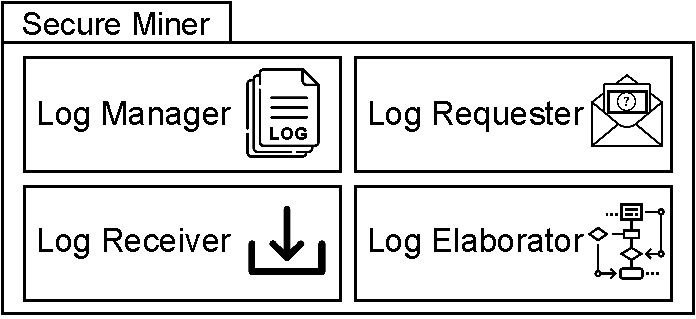
\includegraphics[width=1\textwidth]{content/figures/secureminersad.pdf}
	\caption[Secure Miner sub-components]{Sub-components of the \\Secure Miner}
	\label{fig:trusted_miner}
	\vspace{-6pt}
\end{wrapfigure} 
\noindent\textbf{The Secure Miner.}
The primary objective of the \Compo{Secure Miner} is to allow miners to securely execute process mining algorithms using event logs retrieved from provisioners such as the \Actor{Specialized clinic}, \Actor{Pharmaceutical company}, and the \Actor{Hospital} in our example. \Compo{Secure Miner}s are isolated components that guarantee data inalterability and confidentiality. In \cref{fig:trusted_miner}, we show a schematization of the \Compo{Secure Miner}, which consists of four sub-components:
\begin{inparaenum}[\itshape(i)\upshape]
    \item \Compo{Log Requester};
    \item \Compo{Log Receiver};
    \item \Compo{Log Manager}; 
    \item \Compo{Log Elaborator}.
\end{inparaenum}
%Event logs belonging to provisioners are locked in the \Compo{Secure Miner}.
%We handle  data via the 
The \Compo{Log Requester} and the \Compo{Log Receiver} are the sub-components that we employ during the \NewJ{log partition} retrieval. \Compo{Log Requester}s send authenticable data requests to the \Compo{Log Provider}s. The \Compo{Log Receiver} collects \NewJ{log partitions} sent by \texttt{Log Providers} and entrusts them to the \Compo{Log Manager}, securing them from accesses that are external to the \Compo{Secure Miner}.
Miners of our motivating scenario, such as the \Actor{University} and the \Actor{National Institute of Statistics}, employ these three components to retrieve and store Alice and Bob's data. %The \Compo{Log Elaborator} merges the event data locked in the \Compo{Secure Miner} to have a global view of the inter-organizational process comprehensive of activities executed by each involved party. 
The \NewJ{\Compo{Log Manager}} combines the event data locked in the \Compo{Secure Miner} to have a global view of the inter-organizational process comprehensive of activities executed by each involved \NewJ{provisioning} party. \NewJ{We refer to this operation as \emph{merge}, according to \cref{def:merge}}.
%Thereupon, it 
\NewJ{\Compo{Log Elaborator}} executes process mining algorithms using \NewJ{merged event logs} in a protected environment, inaccessible from the outside computation environment.
%In our motivating scenario, the \Compo{Log Elaborator} combines the traces associated with the cases of Alice (i.e., $T^H_{312}$, $T^S_{312}$, and $T^C_{312}$) and Bob (i.e, $T^H_{711}$, $T^S_{711}$, and $T^C_{711}$) and generates the chronologically sorted traces $T_{312}$ and $T_{711}$ \NewJ{according to their \emph{timestamp} (as described in \cref{post:order:timestamp})}, and feeds them into the mining algorithms (see the bottom of \cref{tab:trace}).
In our motivating scenario, the \Compo{Log Manager} combines the traces associated with the cases of Alice (i.e., $T^H_{312}$, $T^S_{312}$, and $T^C_{312}$) and Bob (i.e, $T^H_{711}$, $T^S_{711}$, and $T^C_{711}$) and generates the chronologically sorted traces $T_{312}$ and $T_{711}$ \NewJ{preserving the events' temporal sequence (as described in \cref{post:order:timestamp}). Subsequently, The \Compo{Log Elaborator} feeds these cases into the mining algorithms.} Thus far, we have outlined the main functionalities of each component at large. Next, we provide the details of the CONFINE protocol and prototype implementation.



